\documentclass[border=4pt]{standalone}
% Shared style for the workflow figures (standalone TikZ, compiled to PDF).
\usepackage[T1]{fontenc}
\usepackage[scaled=0.95]{helvet}
\renewcommand{\familydefault}{\sfdefault}
\usepackage{amsmath,amssymb}
\usepackage{xcolor}
\usepackage{tikz}
\usetikzlibrary{arrows.meta,positioning,calc,fit,backgrounds,shapes.misc,shapes.geometric}

\definecolor{cBlue}{HTML}{2B6CB0}
\definecolor{cTeal}{HTML}{1C8C8C}
\definecolor{cGreen}{HTML}{2F855A}
\definecolor{cPurple}{HTML}{6B46C1}
\definecolor{cOrange}{HTML}{C05621}
\definecolor{cRed}{HTML}{C53030}
\definecolor{cGray}{HTML}{4A5568}
\definecolor{cInk}{HTML}{1A202C}

\tikzset{
  cardbody/.style={rectangle, rounded corners=3pt, line width=0.9pt, align=left,
                   font=\scriptsize\color{cInk}, inner xsep=5pt, inner ysep=5pt},
  cardhead/.style={rectangle, rounded corners=3pt, align=left, text=white,
                   font=\footnotesize, inner xsep=4pt, inner ysep=3.5pt},
  numc/.style={circle, line width=0.9pt, inner sep=0pt, minimum size=5.2mm,
               font=\footnotesize\bfseries},
  flow/.style={-{Stealth[length=2.6mm,width=2.2mm]}, line width=1.3pt, color=cGray},
  loop/.style={-{Stealth[length=2.4mm,width=2mm]}, line width=1.1pt, dashed, color=cRed},
  tag/.style={rectangle, rounded corners=2pt, font=\scriptsize\bfseries, inner sep=2.5pt},
  note/.style={font=\scriptsize\itshape, color=cGray, align=center},
  band/.style={rectangle, rounded corners=6pt, line width=0.8pt, inner sep=7pt},
}

% \card{name}{position}{colour}{number}{title}{body}{width}{body height}
\newcommand{\card}[8]{%
  \node[cardbody, draw=#3, fill=#3!5, text width=#7, minimum height=#8, anchor=north]
       (#1) at (#2) {#6};
  \node[cardhead, fill=#3, text width=#7, anchor=south, yshift=-1.5pt] (#1h) at (#1.north) {\hspace*{4.2mm}\textbf{#5}};
  \node[numc, fill=white, draw=#3, text=#3] at ([xshift=1pt]#1h.west) {#4};
}
\newcommand{\bul}{\textcolor{cGray}{\textbullet}~}

\begin{document}
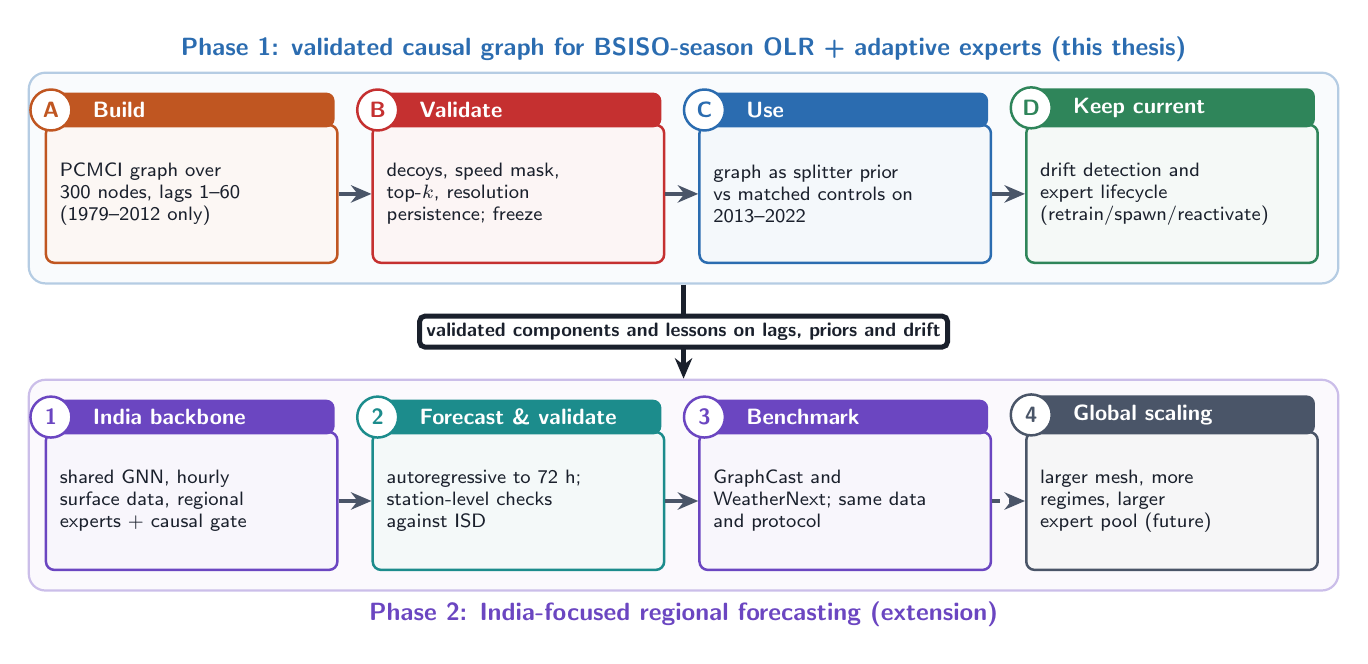
\begin{tikzpicture}
\def\W{3.35cm}\def\H{1.75cm}\def\dx{4.15}
\card{a}{0,0}{cOrange}{A}{Build}{PCMCI graph over\\300 nodes, lags 1--60\\(1979--2012 only)}{\W}{\H}
\card{b}{\dx,0}{cRed}{B}{Validate}{decoys, speed mask,\\top-$k$, resolution\\persistence; freeze}{\W}{\H}
\card{c}{2*\dx,0}{cBlue}{C}{Use}{graph as splitter prior\\vs matched controls on\\2013--2022}{\W}{\H}
\card{d}{3*\dx,0}{cGreen}{D}{Keep current}{drift detection and\\expert lifecycle\\(retrain/spawn/reactivate)}{\W}{\H}
\foreach \x/\y in {a/b,b/c,c/d}{\draw[flow] (\x.east) -- (\y.west);}
\card{p1}{0,-3.9}{cPurple}{1}{India backbone}{shared GNN, hourly\\surface data, regional\\experts + causal gate}{\W}{\H}
\card{p2}{\dx,-3.9}{cTeal}{2}{Forecast \& validate}{autoregressive to 72 h;\\station-level checks\\against ISD}{\W}{\H}
\card{p3}{2*\dx,-3.9}{cPurple}{3}{Benchmark}{GraphCast and\\WeatherNext; same data\\and protocol}{\W}{\H}
\card{p4}{3*\dx,-3.9}{cGray}{4}{Global scaling}{larger mesh, more\\regimes, larger\\expert pool (future)}{\W}{\H}
\foreach \x/\y in {p1/p2,p2/p3}{\draw[flow] (\x.east) -- (\y.west);}
\draw[flow, dashed] (p3.east) -- (p4.west);
\begin{scope}[on background layer]
\node[band, draw=cBlue!35, fill=cBlue!3, fit=(ah)(d), label={[font=\small\bfseries\color{cBlue}]above:Phase 1: validated causal graph for BSISO-season OLR + adaptive experts (this thesis)}] (P1) {};
\node[band, draw=cPurple!35, fill=cPurple!3, fit=(p1h)(p4), label={[font=\small\bfseries\color{cPurple}]below:Phase 2: India-focused regional forecasting (extension)}] (P2) {};
\end{scope}
\draw[flow, line width=1.8pt, color=cInk] (P1.south) -- node[tag, draw=cInk, fill=white, text=cInk]{validated components and lessons on lags, priors and drift} (P2.north);
\end{tikzpicture}
\end{document}
